\section{Designing a Traffic Shaping Tunnel}
\label{sec:netshaper-designing-traffic-shaping-tunnel}

A traffic-shaping tunnel must satisfy the following requirements.
\textbf{First}, the tunnel should satisfy DP guarantees.
For this, the tunnel should complete a DP query and prepare shaped packets containing the data (and padding, if necessary) within a finite interval.
It must also be able to transmit the shaped packets within the same interval.
\textbf{Second}, no adversary should be able to distinguish between the data and the padding.
For this, both data and padding should be identical with respect to their network behaviour (i.e. congestion control, loss recovery, and acknowledgements).
\textbf{Third}, the tunnel must provide similar levels of reliability, congestion control, and loss recovery as the end host application expects.

\Cref{fig:tunnel-endpoint-design} outlines the design of one endpoint of the tunnel. A similar endpoint is deployed on the other side of the tunnel.
The tunnel endpoints establish a bidirectional, encrypted QUIC connection that carries both the payload bytes from one or more applications and the dummy bytes.
The endpoints contain a shaping layer (Shaper), which determines the DP amount of bytes to be sent out in the given finite interval and sends it out using the already established QUIC connection.

\begin{figure}[!htb]
    \centering
    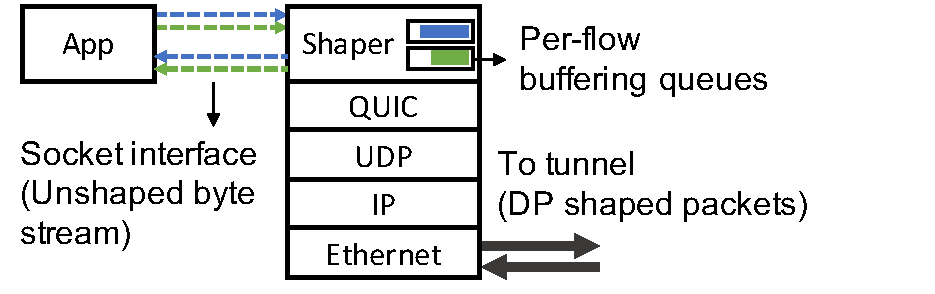
\includegraphics[width=\columnwidth]{figures/netshaper/tunnel-endpoint-design.pdf}
    \caption{Overview of tunnel design (one endpoint)}
    \label{fig:tunnel-endpoint-design}
\end{figure}

NetShaper adopts a transport-layer proxy tunnel architecture, where each end host application terminates the connection at its local tunnel endpoint (see \Cref{fig:netshaper-setup}). Hence, each communication byte stream traverses through three piecewise connections: (i) Between the application and the local tunnel endpoint, (ii) between the tunnel endpoints, and (iii) between the remote tunnel endpoint and the remote application.

\begin{figure}[!htb]
    \centering
    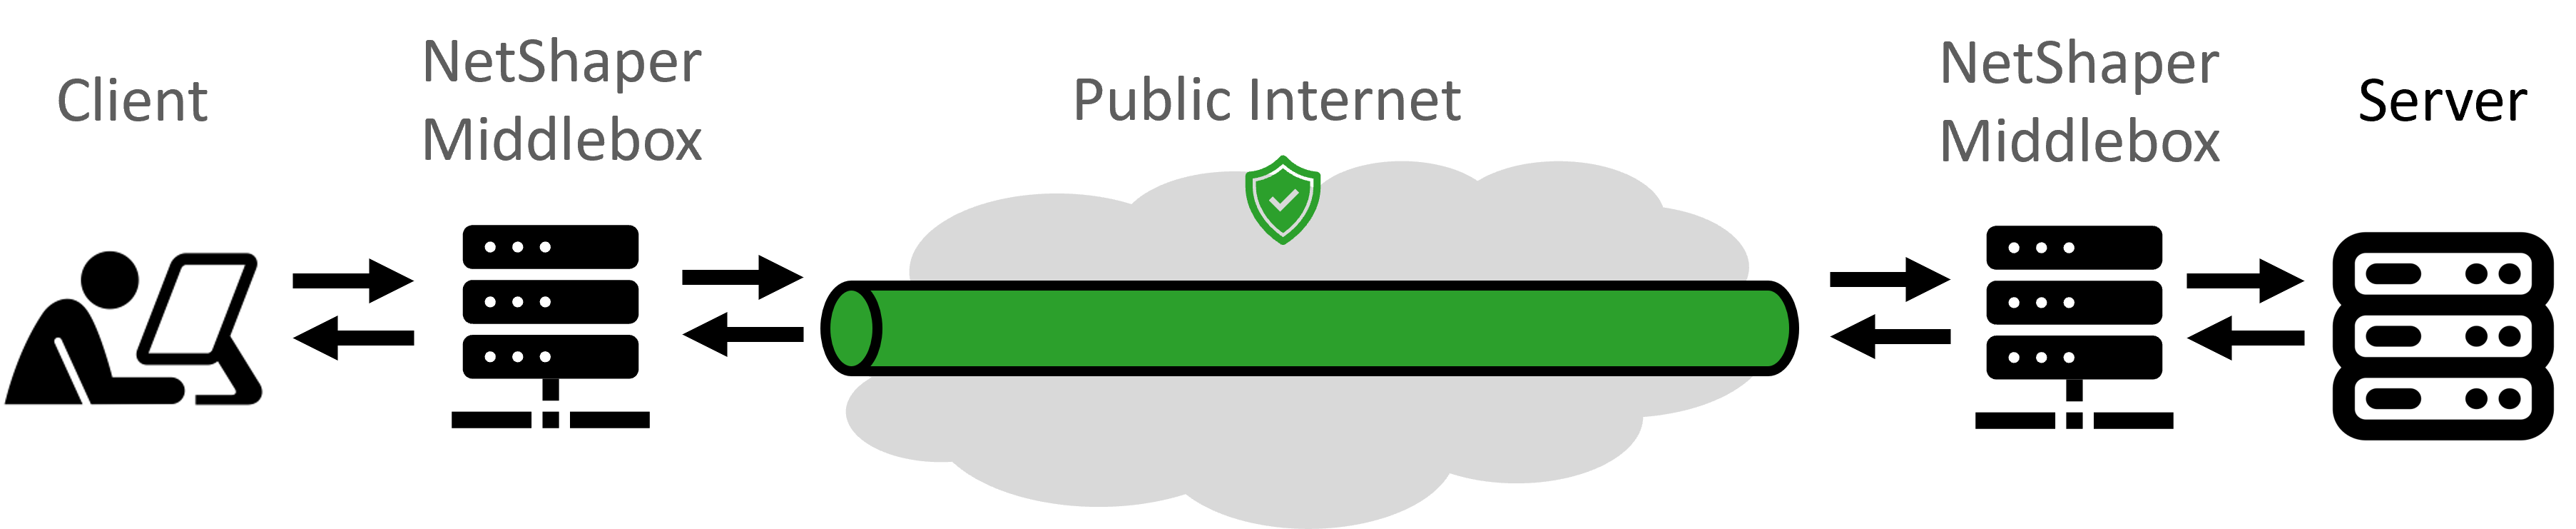
\includegraphics[width=\columnwidth]{figures/netshaper/netshaper-setup.png}
    \caption{NetShaper's Tunnel Setup}
    \label{fig:netshaper-setup}
\end{figure}

\paragraph{Scaling with multiple end hosts.}
In order to amortise the overhead and scale with multiple end hosts, the tunnel can rely on QUIC streams (see \Cref{subsec:netshaper-background-quic})
Using this, the tunnel can proxy the payload of multiple end hosts through a single QUIC connection between a pair of middleboxes.

While QUIC can support arbitrary initialisation and termination of streams, each stream has an associated header, which would increase the total transmission size.
For example, when transmitting $n$ bytes in a single stream, the total transmission size would be $n + S_{header}$.
However, when transmitting $k$ streams of $n/k$ byte each, the total transmission size would be $n + k*S_{header}$. 
An adversary may be able to distinguish between these two scenarios.
In order to avoid such a situation, the tunnel must initialise a fixed number of streams per QUIC connection during the setup phase, and not establish any more streams once the tunnel is established.


\subsection{Tunnel Operations}

\paragraph{Tunnel setup and teardown.}
In order to communicate securely using NetShaper's tunnel, the application first needs to send a configuration message to its local tunnel endpoint.
The configuration message contains the privacy parameters, the source and destination (IP and port), and a reliability flag determining whether the tunnel should provide reliable delivery semantics.
Next, the tunnel endpoint needs to establish a QUIC connection with the tunnel endpoint on the destination side and configure the privacy parameters for that connection
\footnote{A new connection may not be established if an existing connection with similar parameters offering similar or better privacy guarantees already exists.}.
The local tunnel endpoint also establishes three types of QUIC streams: control, data and dummy.
One \textit{control stream} is used to transmit messages regarding connection establishment or termination by an endpoint.
\textit{dummy stream} is used to transmit the dummy/padding whenever the DP query results in more bytes than available from the sending application
\footnote{We do not use QUIC's PADDING frames as they do not elicit acknowledgements, and hence, are distinguishable on the network \cite{quic_rfc}.}.
One or more \textit{data streams}, each carrying the data/payload of one application.

The tunnel is configured with an idle timeout, after which one endpoint initiates the termination sequence and shuts down the established QUIC streams and the QUIC connection.

\paragraph{End host connection establishment and termination.}
Once the tunnel setup is complete, the end host applications can establish or terminate connections with each other.
Whenever an end host application establishes a connection, the Shaper maps this connection to a QUIC \textit{data stream}.
It then transmits a message of connection establishment containing the source, the destination, and the ID of the associated \textit{data stream} on the \textit{control stream}.
The remote tunnel establishes a new connection to the remote application based on the connection establishment message and maps this connection to the relevant \textit{data stream}.
Similarly, whenever an end host terminates a connection, the Shaper transmits a connection termination message on the \textit{control stream}, and the remote end host terminates the connection with the remote application after ensuring all pending data has been transmitted.

\paragraph{Outbound traffic shaping.}
The Shaper accumulates the application byte streams in buffering queues.
At the start of every finite interval, the Shaper measures the total size of the available data in the buffering queues ($L$). 
It then adds some noise $\eta$ to this size based on the configured privacy (DP) parameters.
Hence, the total size to be transmitted in this window is $L + \eta$.
In the same interval, it also prepares the \textit{shaped buffer} that contains $R$ payload bytes and $D = max(0, L + \eta - R)$ dummy bytes and enqueues it for QUIC to transmit.
QUIC then takes this buffer and prepares QUIC packets based on the constraints on the connection (e.g. maximum transmission unit, congestion window size, and flow window size).
Then, QUIC sends these prepared packets out by using the networking stack's UDP layer.

\paragraph{Inbound traffic processing.}
For incoming shaped packets, QUIC sends an ACK to the sender and decrypts the packet.
The tunnel endpoint then processes the decrypted packet, drops the dummy bytes, and forwards the application data byte streams to the relevant remote applications.

\endinput